%! TEX root = ../main.tex
% =============================================================
% IMMUTABLE — generated automatically, do not edit this block
%   script          : analysis_scratch/sliding_afft_fullwind_sweep.py
%   plot_type       : sliding_afft_stability
%   chapter         : 04
%   probe           : 9373/170
%   window_s        : 15.0
% =============================================================
\begin{figure}[htbp]
  \centering
  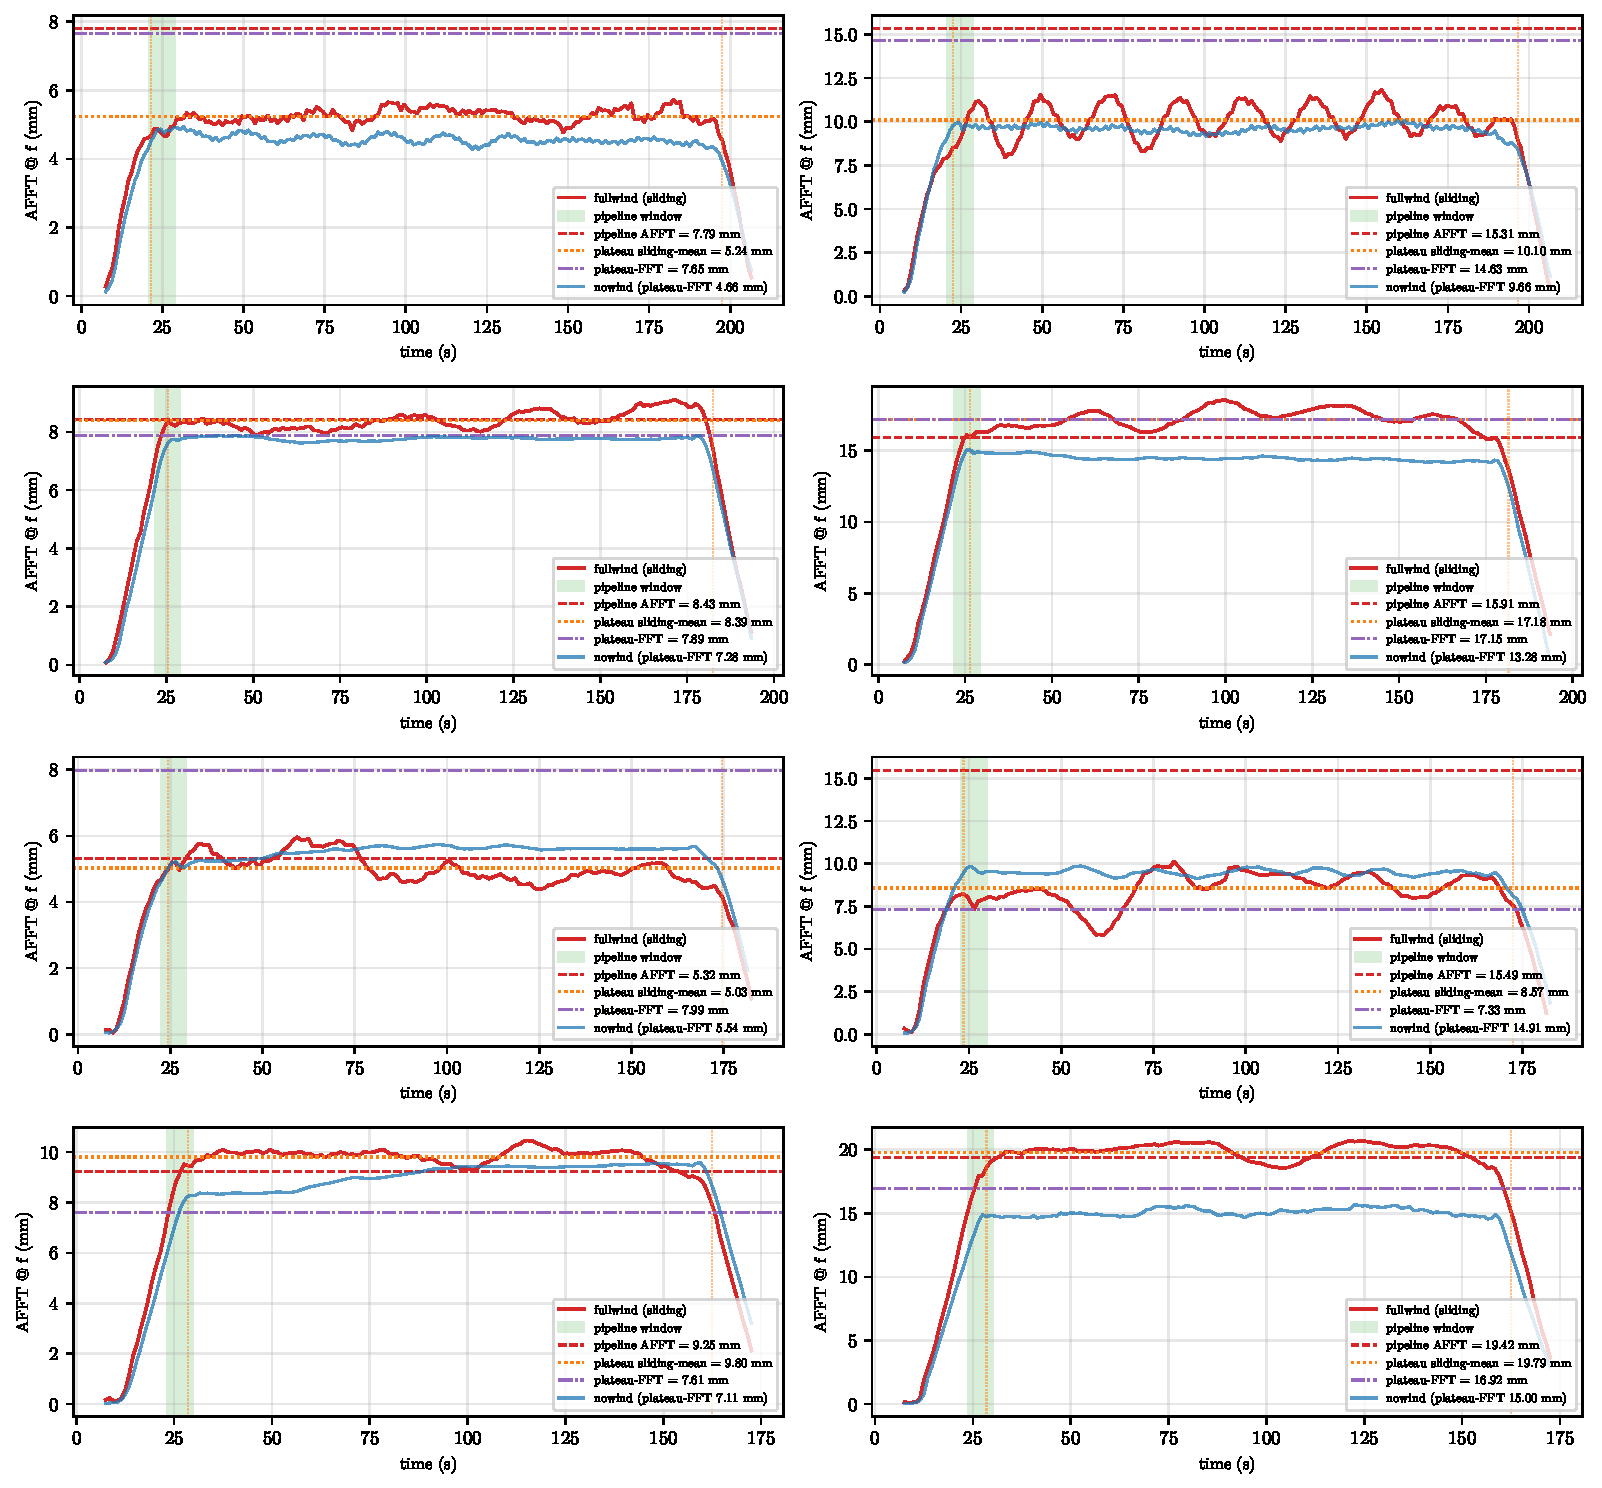
\includegraphics[width=\linewidth]{FIGURES/ch04_sliding_afft_stability.pdf}
  \caption[Sliding-window FFT at the IN probe]{%
    Sliding-window FFT at the IN probe (9373/170) for fullwind per240 wave runs at 1.3--1.6 Hz, 0.1/0.2 V. Each panel: red = fullwind run, blue = nowind reference, green band = pipeline analysis window. Dashed red = pipeline AFFT; orange dotted = mean over the alive plateau; purple dash-dot = one-shot FFT over the full plateau. The sliding AFFT is stable across the run in 7/8 conditions (no within-run transient). Apparent discrepancies between pipeline AFFT and plateau-FFT reflect FFT bin-grid alignment (see CH04 \S4b), not physical signal variation. Window = 15\,s, step = 1\,s, bin search = $\pm$0.10\,Hz.
  }
  \label{fig:ch04_sliding_afft_stability}
\end{figure}
